% Full instructions available at:
% https://github.com/elauksap/focus-beamertheme

\documentclass{beamer}
\usetheme{focus}
\usepackage[absolute,overlay]{textpos}
\usepackage{graphicx}

\title{Introducción a GIT}
\subtitle{El mejor amigo de un desarrollador}
\author{Por: Enrique Walter Philippeaux}
\date{}

\begin{document}
    \begin{frame}
        \begin{textblock*}{.5\textwidth}(6.5cm,8cm) % {block width} (coords)
        
\includegraphics[width=\textwidth]{logochicogris.pdf}
        \end{textblock*}
        
        \begin{textblock*}{3cm}(0.5cm,7.9cm) % {block width} (coords)
        
\includegraphics[width=3cm]{gitlogogris.pdf}
        \end{textblock*}
        \maketitle
    \end{frame}
    
    
    \section{Algo muy común...}
    \begin{frame}{Algo muy común...}
    ¿Alguna vez les paso?\pause
    \begin{enumerate}
        \item \textsc{Entrega}\pause
        \item \textsc{Entrega Final}\pause
        \item \textsc{Entrega final2}\pause
        \item \textsc{Entrega finalok}\pause
        \item \textsc{Entrega finalisima}\pause
        \item \textsc{Entrega finalahorasi}\pause
        \item \textsc{Entrega FINAL}\pause
        \item \textsc{Entrega finalasd}\pause
        \item \textsc{EntregAAAAAAAAAA}
    \end{enumerate}
    \end{frame}
    
    %levante la mano quien le ha ocurrido algo similar...
    
    %2 minutos y medio,
    %Trabajo en ROBOT SUMO, bahia blanca: donde "perdimos" el código simple que "solo funcionaba" y no pudimos utilizar el algoritmo completo.
    %Tuvimos que cambiar de microcontrolador....
    
    \section{¿Qué es GIT?}
    \begin{frame}{¿Qué es GIT?}
        \begin{textblock*}{3cm}(9cm,7.5cm) % {block width} (coords)
        
\includegraphics[width=3cm]{gitlogo.pdf}
        \end{textblock*}
        \begin{itemize}
            \item Git es un \textbf{Sistema de Control de Versiones}.\\\pause
            \begin{itemize}
                \item Facilita mantener múltiples versiones de un proyecto.\pause
                \item Facilita la interacción entre múltiples desarrolladores.\pause
                \item Previene la pérdida de información entre versiones.\pause
            \end{itemize}
            \item Nos permite ver cambios que hicimos en nuestro proyecto, y revertirlos.\pause
            \item No es \textbf{GITHUB}.
        \end{itemize}
    \end{frame}
    
    \section{¿Qué es GitHub?}
    \begin{frame}{¿Qué es GitHub?}
        \begin{textblock*}{3cm}(9cm,7.5cm) % {block width} (coords)
        
\includegraphics[width=3cm]{GitHub_Logo.png}
        \end{textblock*}
        \begin{itemize}
            \item \textbf{Github.com} es un sitio web que \textbf{almacena} repositorios de git, en un \textbf{servidor remoto}.\pause
            \item Facilita compartir proyectos entre equipos.\pause
            \item Proporciona una interfaz gráfica amigable\pause
            \item Es gratis.
        \end{itemize}
    \end{frame}
    
    \section{¿Donde utilizamos GIT?}
    \begin{frame}{¿Donde utilizamos GIT?}
        \begin{textblock*}{3cm}(9cm,6cm) % {block width} (coords)
        
\includegraphics[width=3cm]{idea.png}
        \end{textblock*}
        \pause
        \begin{itemize}
            \item Códigos fuente\pause
            \item Documentos\pause
            \item Desarrollos electrónicos\pause
            \item Proyecto Final/Tesis
        \end{itemize}
    \end{frame}
    
    \section{¿Cómo se configura?}
    \begin{frame}{¿Cómo se configura?}
        Nuestros \textbf{commits} llevan consigo los siguientes datos:\pause
        \begin{itemize}
            \item Nombre del autor\pause\\
            \texttt{\$ git config --global user.name "Juan Perez"}\pause
            \item Email del autor\pause\\
            \texttt{\$ git config --global user.email "jp@git.com"}\pause
            \item Fecha y hora\pause\\
            Este es automático..
        \end{itemize}
    \end{frame}
    
    \section{Utilizando git}
    \begin{frame}{Utilizando git}
        \begin{itemize}
            \item Creamos/Nos situamos en la carpeta de nuestro proyecto\pause
            \begin{block}{\texttt{git init}}
                Inicializamos el \textbf{repositorio} de git
            \end{block}\pause
            \begin{block}{\texttt{git clone url}}
                Si queremos trabajar sobre un \textbf{repositorio existente}, lo clonamos.
            \end{block}
        \end{itemize}
    \end{frame}
    \begin{frame}{Utilizando git}
        \begin{itemize}
            \item Agregamos y trabajamos sobre nuestros archivos\pause
            \begin{block}{\texttt{git add .}}
                Añadimos los nuevos cambios
            \end{block}\pause
            \begin{block}{\texttt{git commit -m "mensaje :)"}}
                Creamos un \textbf{commit}
            \end{block}
        \end{itemize}
    \end{frame}
    \begin{frame}{Utilizando git}
        Teniendo nuestro repositorio podemos vincularlo a \textbf{Github}.
        \begin{itemize}
            \item Creamos nuestro \textbf{repositorio} en \textbf{Github}\pause
            \item Seguimos las instrucciones en \textbf{Github} para conectar nuestro \textbf{repositorio} a su \textbf{servidor remoto}.\pause
            \begin{block}{\texttt{git push origin}}
                Subimos nuestros cambios al \textbf{servidor remoto}
            \end{block}
        \end{itemize}
    \end{frame}
    \section{Ramas/Branches}
    \begin{frame}{¿Qué es una rama?}
        Según \textit{Atlassian}:\pause
        \begin{itemize}
            \item Son parte del proceso de desarrollo diario.\pause
            \item Son un puntero a las instantáneas de nuestros cambios.\pause
            \item Las utilizamos al agregar nuevas funciones, o solucionar errores.
        \end{itemize}
    \end{frame}
    \begin{frame}{Diagrama ejemplar}
        \begin{center}
            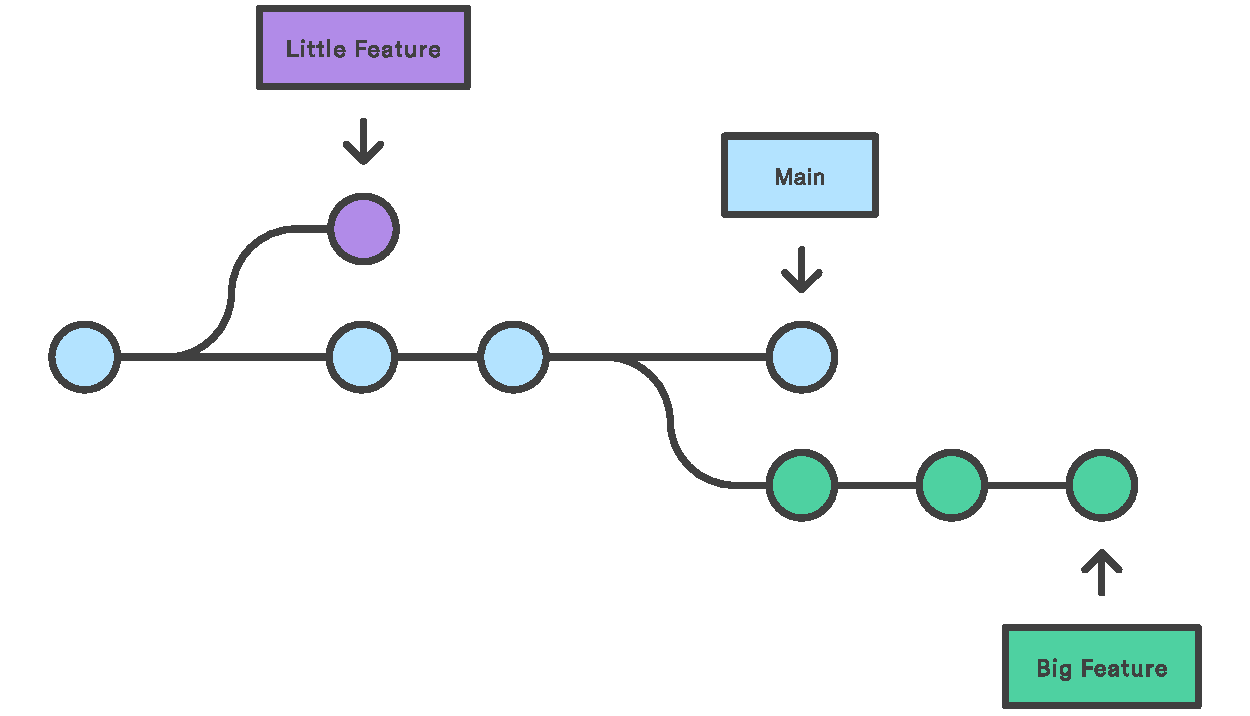
\includegraphics[width=\textwidth]{01 Git branch.pdf}
        \end{center}
    \end{frame}
    \begin{frame}{Comandos útiles}
        \begin{block}{\texttt{git branch}}
            \textbf{Enumera} todas las ramas de tu repositorio
        \end{block}\pause
        \begin{block}{\texttt{git checkout <nombre>}}
            Nos \textbf{situa} en la rama llamada \texttt{<nombre>}
        \end{block}\pause
        \begin{block}{\texttt{git checkout -b <nueva>}}
            \textbf{Crea} una nueva rama llamada \texttt{<nueva>}
        \end{block}\pause
        \begin{block}{\texttt{git branch -D <test>}}
            \textbf{Borra} la rama llamada \texttt{<test>}
        \end{block}
    \end{frame}
    
    \section{Fusión/Merge}
    \begin{frame}{¿Qué es un Merge?}
        \begin{center}
            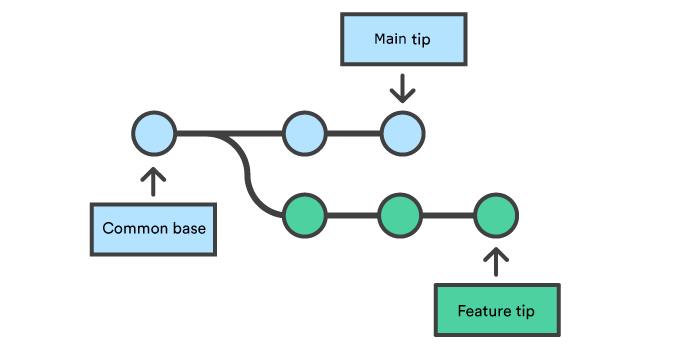
\includegraphics[width=\textwidth]{01 Branch-2 kopiera.png}
        \end{center}
    \end{frame}
    \begin{frame}{¿Qué es un Merge?}
        \begin{center}
            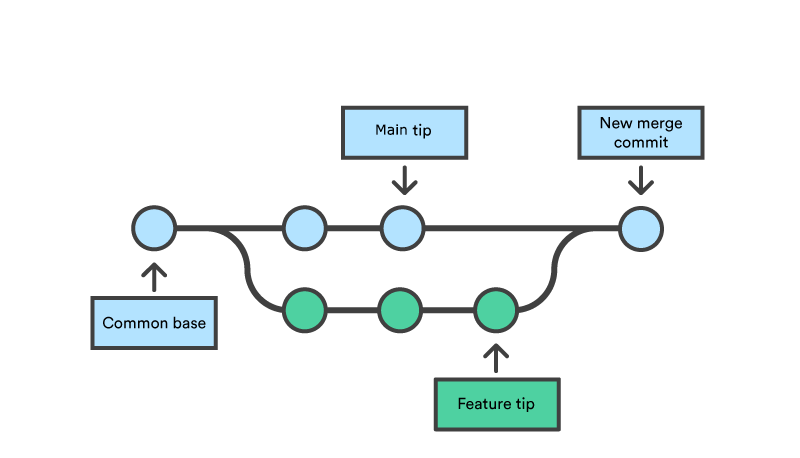
\includegraphics[width=\textwidth]{02 Branch-1 kopiera.png}
        \end{center}
    \end{frame}
    \begin{frame}{Flujo de trabajo}
        \begin{block}{\texttt{git checkout feature}}
            Nos situamos en la \textbf{rama feature}
        \end{block}\pause
        Ahora realizo mis cambios en la rama...\pause
        \begin{block}{\texttt{git add .}}
            \textbf{Agregamos} nuestros cambios
        \end{block}\pause
        \begin{block}{\texttt{git commit -m "mensaje"}}
            Creamos un \textbf{commit}.
        \end{block}\pause
        \begin{block}{\texttt{git merge feature main}}
            Fusionamos los cambios que hicimos en la rama \textbf{feature} a la rama principal: \textbf{main}.
        \end{block}
    \end{frame}
    
    \begin{frame}{Resumen}
    \begin{enumerate}
        \item La fusión en git combina secuencias de cambios en un solo historial unificado\pause
        \item Git permite fusionar las confirmaciones automáticamente salvo que haya \textbf{conflictos}
    \end{enumerate}
    \end{frame}
    
    
    \section{Conflictos}
    \begin{frame}{Conflictos}
    \begin{itemize}
        \item Los conflictos emergen cuando dos miembros del mismo equipo de desarrollo\pause  trabajan en el \textbf{mismo archivo}\pause  e intentan \textbf{fusionar} sus cambios.\pause
        \item La manera mas eficiente de \textbf{evitarlos} es trabajar en \textbf{ramas separadas}\pause  y esperar que el otro desarrollador suba sus cambios a la rama \textbf{main}\pause  para \textbf{Integrarlos} en mi rama de trabajo, y subir los mios.\pause
        \item Si surgen conflictos, ¡No se preocupen!\pause\\Siempre y cuando trabajemos con archivos de texto.
    \end{itemize}
    \end{frame}
    \begin{frame}{Resolviendo un conflicto en VSCode}
        \begin{center}
            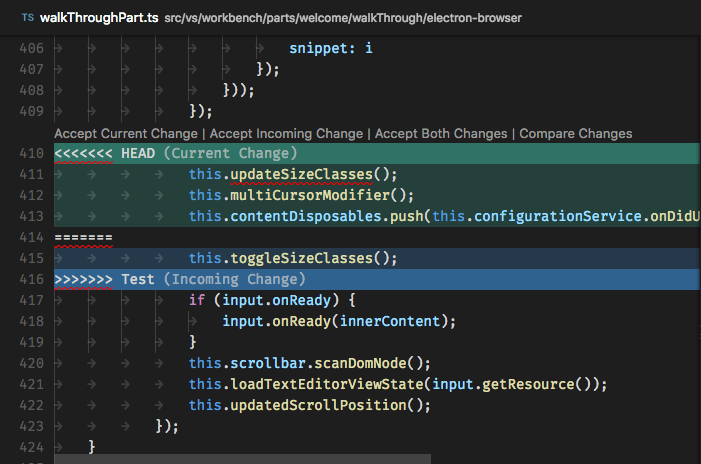
\includegraphics[width=\textwidth]{merge-conflict.png}
        \end{center}
    \end{frame}
    
    \section{Etiquetas/tags}
    \begin{frame}{¿Qué es una etiqueta?}
    \pause
        \begin{itemize}
            \item Una referencia a un punto específico de la historia del repositorio.\pause
            \item Se utiliza para capturar un punto, y marcar una "versión".\pause
            \item Es una rama que \textbf{no cambia}.
        \end{itemize}
    \end{frame}
    \begin{frame}{Comandos útiles}
        \begin{block}{\texttt{git tag}}
            Nos muestra la lista de etiquetas del repositorio.
        \end{block}\pause
        \begin{block}{\texttt{git tag <nombre>}}
            Crea una nueva etiqueta desde \textbf{mi punto actual}, llamada \texttt{<nombre>}
        \end{block}\pause
        \begin{block}{\texttt{git tag -a <nombre> -m "descripcion"}}
            Crea una nueva etiqueta desde \textbf{mi punto actual}, llamada \texttt{<nombre>}, incluyendo una descripcion a preferencia.
        \end{block}\pause
        \begin{block}{\texttt{git checkout v1.4}}
            Nos situa en la \textbf{etiqueta} \texttt{"v1.4"}, tal como si fuera una \textbf{rama}.
        \end{block}
    \end{frame}
    
    \section{Terminando...}
    \begin{frame}{Recursos Útiles}
        \begin{itemize}
            \item Tutorial de Atlassian acerca de \textbf{git}:\\
            \texttt{https://www.atlassian.com/es/git/tutorials}
            \item Integración nativa en \textbf{VSCode}:\\
            \texttt{https://code.visualstudio.com/}
            \item Cliente de \textbf{GitHub}\\
            \texttt{https://desktop.github.com/}
        \end{itemize}
    \end{frame}
    \begin{frame}[plain]{¡Gracias por participar!}
        \begin{center}
            \huge{¡Gracias por participar!}
            
\includegraphics[width=\textwidth]{qr-conlogo.pdf}
        \end{center}
    \end{frame}
    
    
    %Referir al tutorial https://www.atlassian.com/es/git/tutorials
\end{document}
